\PassOptionsToPackage{unicode=true}{hyperref} % options for packages loaded elsewhere
\PassOptionsToPackage{hyphens}{url}
%
\documentclass[
]{article}
\usepackage{lmodern}
\usepackage{amssymb,amsmath}
\usepackage{ifxetex,ifluatex}
\ifnum 0\ifxetex 1\fi\ifluatex 1\fi=0 % if pdftex
  \usepackage[T1]{fontenc}
  \usepackage[utf8]{inputenc}
  \usepackage{textcomp} % provides euro and other symbols
\else % if luatex or xelatex
  \usepackage{unicode-math}
  \defaultfontfeatures{Scale=MatchLowercase}
  \defaultfontfeatures[\rmfamily]{Ligatures=TeX,Scale=1}
\fi
% use upquote if available, for straight quotes in verbatim environments
\IfFileExists{upquote.sty}{\usepackage{upquote}}{}
\IfFileExists{microtype.sty}{% use microtype if available
  \usepackage[]{microtype}
  \UseMicrotypeSet[protrusion]{basicmath} % disable protrusion for tt fonts
}{}
\makeatletter
\@ifundefined{KOMAClassName}{% if non-KOMA class
  \IfFileExists{parskip.sty}{%
    \usepackage{parskip}
  }{% else
    \setlength{\parindent}{0pt}
    \setlength{\parskip}{6pt plus 2pt minus 1pt}}
}{% if KOMA class
  \KOMAoptions{parskip=half}}
\makeatother
\usepackage{xcolor}
\IfFileExists{xurl.sty}{\usepackage{xurl}}{} % add URL line breaks if available
\IfFileExists{bookmark.sty}{\usepackage{bookmark}}{\usepackage{hyperref}}
\hypersetup{
  pdftitle={Homework1\_Question1},
  pdfauthor={Hannah Zmuda},
  pdfborder={0 0 0},
  breaklinks=true}
\urlstyle{same}  % don't use monospace font for urls
\usepackage[margin=1in]{geometry}
\usepackage{color}
\usepackage{fancyvrb}
\newcommand{\VerbBar}{|}
\newcommand{\VERB}{\Verb[commandchars=\\\{\}]}
\DefineVerbatimEnvironment{Highlighting}{Verbatim}{commandchars=\\\{\}}
% Add ',fontsize=\small' for more characters per line
\usepackage{framed}
\definecolor{shadecolor}{RGB}{248,248,248}
\newenvironment{Shaded}{\begin{snugshade}}{\end{snugshade}}
\newcommand{\AlertTok}[1]{\textcolor[rgb]{0.94,0.16,0.16}{#1}}
\newcommand{\AnnotationTok}[1]{\textcolor[rgb]{0.56,0.35,0.01}{\textbf{\textit{#1}}}}
\newcommand{\AttributeTok}[1]{\textcolor[rgb]{0.77,0.63,0.00}{#1}}
\newcommand{\BaseNTok}[1]{\textcolor[rgb]{0.00,0.00,0.81}{#1}}
\newcommand{\BuiltInTok}[1]{#1}
\newcommand{\CharTok}[1]{\textcolor[rgb]{0.31,0.60,0.02}{#1}}
\newcommand{\CommentTok}[1]{\textcolor[rgb]{0.56,0.35,0.01}{\textit{#1}}}
\newcommand{\CommentVarTok}[1]{\textcolor[rgb]{0.56,0.35,0.01}{\textbf{\textit{#1}}}}
\newcommand{\ConstantTok}[1]{\textcolor[rgb]{0.00,0.00,0.00}{#1}}
\newcommand{\ControlFlowTok}[1]{\textcolor[rgb]{0.13,0.29,0.53}{\textbf{#1}}}
\newcommand{\DataTypeTok}[1]{\textcolor[rgb]{0.13,0.29,0.53}{#1}}
\newcommand{\DecValTok}[1]{\textcolor[rgb]{0.00,0.00,0.81}{#1}}
\newcommand{\DocumentationTok}[1]{\textcolor[rgb]{0.56,0.35,0.01}{\textbf{\textit{#1}}}}
\newcommand{\ErrorTok}[1]{\textcolor[rgb]{0.64,0.00,0.00}{\textbf{#1}}}
\newcommand{\ExtensionTok}[1]{#1}
\newcommand{\FloatTok}[1]{\textcolor[rgb]{0.00,0.00,0.81}{#1}}
\newcommand{\FunctionTok}[1]{\textcolor[rgb]{0.00,0.00,0.00}{#1}}
\newcommand{\ImportTok}[1]{#1}
\newcommand{\InformationTok}[1]{\textcolor[rgb]{0.56,0.35,0.01}{\textbf{\textit{#1}}}}
\newcommand{\KeywordTok}[1]{\textcolor[rgb]{0.13,0.29,0.53}{\textbf{#1}}}
\newcommand{\NormalTok}[1]{#1}
\newcommand{\OperatorTok}[1]{\textcolor[rgb]{0.81,0.36,0.00}{\textbf{#1}}}
\newcommand{\OtherTok}[1]{\textcolor[rgb]{0.56,0.35,0.01}{#1}}
\newcommand{\PreprocessorTok}[1]{\textcolor[rgb]{0.56,0.35,0.01}{\textit{#1}}}
\newcommand{\RegionMarkerTok}[1]{#1}
\newcommand{\SpecialCharTok}[1]{\textcolor[rgb]{0.00,0.00,0.00}{#1}}
\newcommand{\SpecialStringTok}[1]{\textcolor[rgb]{0.31,0.60,0.02}{#1}}
\newcommand{\StringTok}[1]{\textcolor[rgb]{0.31,0.60,0.02}{#1}}
\newcommand{\VariableTok}[1]{\textcolor[rgb]{0.00,0.00,0.00}{#1}}
\newcommand{\VerbatimStringTok}[1]{\textcolor[rgb]{0.31,0.60,0.02}{#1}}
\newcommand{\WarningTok}[1]{\textcolor[rgb]{0.56,0.35,0.01}{\textbf{\textit{#1}}}}
\usepackage{graphicx,grffile}
\makeatletter
\def\maxwidth{\ifdim\Gin@nat@width>\linewidth\linewidth\else\Gin@nat@width\fi}
\def\maxheight{\ifdim\Gin@nat@height>\textheight\textheight\else\Gin@nat@height\fi}
\makeatother
% Scale images if necessary, so that they will not overflow the page
% margins by default, and it is still possible to overwrite the defaults
% using explicit options in \includegraphics[width, height, ...]{}
\setkeys{Gin}{width=\maxwidth,height=\maxheight,keepaspectratio}
\setlength{\emergencystretch}{3em}  % prevent overfull lines
\providecommand{\tightlist}{%
  \setlength{\itemsep}{0pt}\setlength{\parskip}{0pt}}
\setcounter{secnumdepth}{-2}
% Redefines (sub)paragraphs to behave more like sections
\ifx\paragraph\undefined\else
  \let\oldparagraph\paragraph
  \renewcommand{\paragraph}[1]{\oldparagraph{#1}\mbox{}}
\fi
\ifx\subparagraph\undefined\else
  \let\oldsubparagraph\subparagraph
  \renewcommand{\subparagraph}[1]{\oldsubparagraph{#1}\mbox{}}
\fi

% set default figure placement to htbp
\makeatletter
\def\fps@figure{htbp}
\makeatother


\title{Homework1\_Question1}
\author{Hannah Zmuda}
\date{}

\begin{document}
\maketitle

\hypertarget{question-1}{%
\section{Question 1}\label{question-1}}

The goal of this problem is to find the inverse CDF of the given
density:

\[ f_X(x) = exp(x - e^x)\]

This will be done by creating an algorithm to simulate the standard
extreme value distribution. In order to find the distribution of the
given density, i first find the CDF of the density by integrating the
equation above: \[F_x(x) = -e^{-e^{x}}\] And then take the inverse of
the equation: \[F_x^{-1}(x) = ln(-ln(-x))\]

\begin{Shaded}
\begin{Highlighting}[]
\NormalTok{n <-}\StringTok{ }\DecValTok{1000} \CommentTok{#sample number}
\NormalTok{U1 <-}\StringTok{ }\KeywordTok{runif}\NormalTok{(n,}\DecValTok{0}\NormalTok{,}\DecValTok{1}\NormalTok{) }\CommentTok{#Random Number Generator, numbers are evenly distributed between 0 and 1}
\NormalTok{f <-}\StringTok{ }\ControlFlowTok{function}\NormalTok{(x)\{}\KeywordTok{exp}\NormalTok{(x }\OperatorTok{-}\StringTok{ }\KeywordTok{exp}\NormalTok{(x))\}}\CommentTok{#the standard extreme value distribution density function}
\NormalTok{q <-}\StringTok{ }\ControlFlowTok{function}\NormalTok{(U1)\{}\OperatorTok{-}\KeywordTok{log}\NormalTok{(}\OperatorTok{-}\KeywordTok{log}\NormalTok{(U1))\}}\CommentTok{#inverse of the standard extreme value distribution density function, run uniform data through (U1)}
\CommentTok{#histogram of simulated data}
\KeywordTok{hist}\NormalTok{(}\KeywordTok{q}\NormalTok{(U1), }\DataTypeTok{prob =} \OtherTok{TRUE}\NormalTok{, }\DataTypeTok{main =} \StringTok{"Standard Extreme Value Distibution"}\NormalTok{, }\DataTypeTok{ylim =} \KeywordTok{c}\NormalTok{(}\DecValTok{0}\NormalTok{, }\DecValTok{1}\NormalTok{), }\DataTypeTok{xlab =} \StringTok{"Values"}\NormalTok{, }\DataTypeTok{ylab =}\StringTok{"Density"}\NormalTok{)}
\NormalTok{x <-}\StringTok{ }\KeywordTok{seq}\NormalTok{(}\KeywordTok{min}\NormalTok{(}\KeywordTok{q}\NormalTok{(U1)), }\KeywordTok{max}\NormalTok{(}\KeywordTok{q}\NormalTok{(U1)), }\FloatTok{0.01}\NormalTok{)}
\KeywordTok{lines}\NormalTok{(x,}\KeywordTok{f}\NormalTok{(x), }\DataTypeTok{col =} \StringTok{"blue"}\NormalTok{) }\CommentTok{#density curve of f(x)}

\KeywordTok{box}\NormalTok{()}
\end{Highlighting}
\end{Shaded}

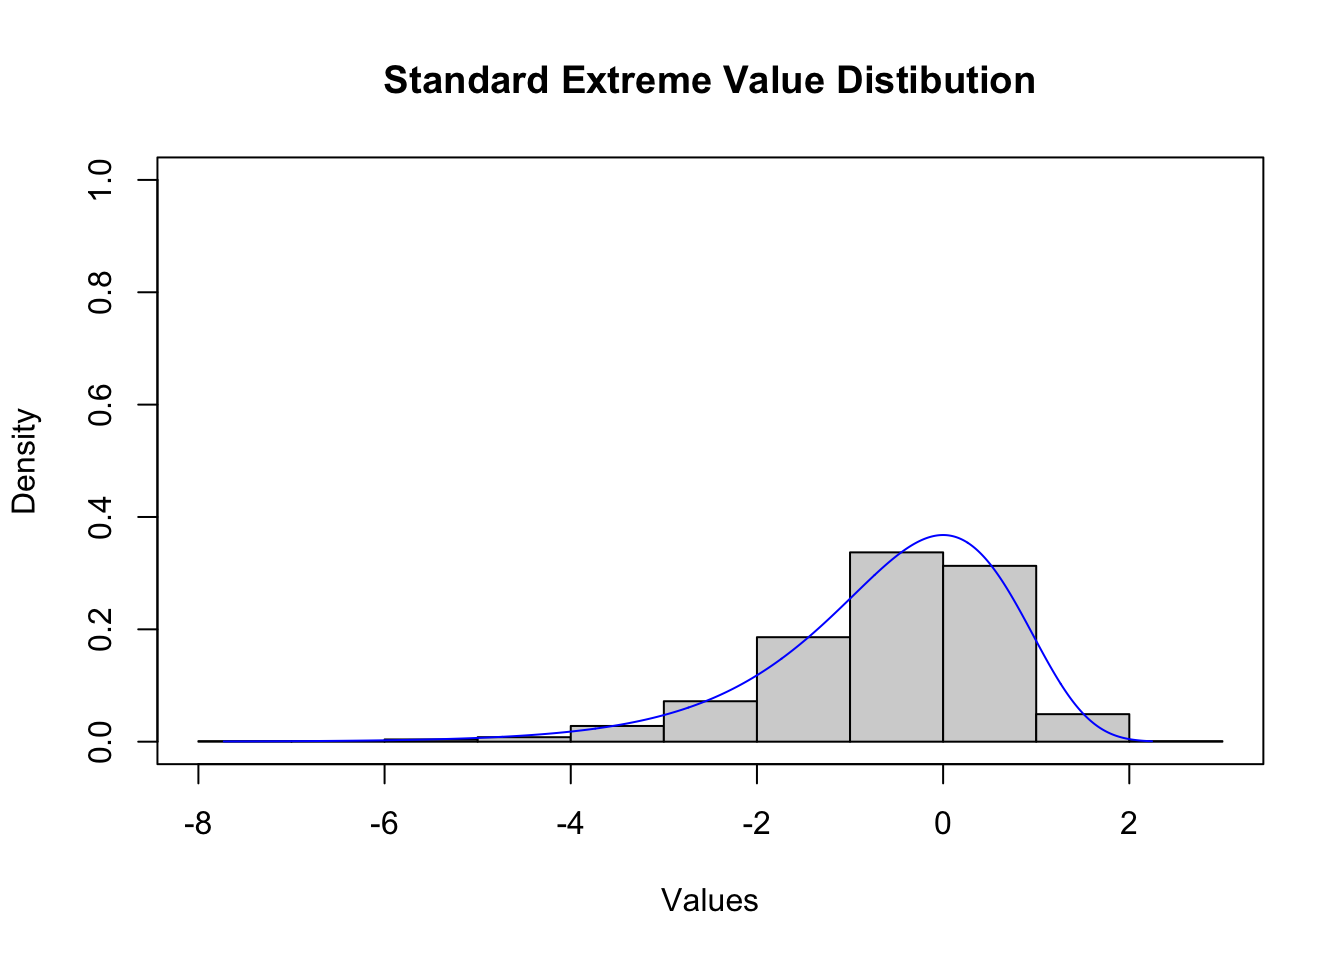
\includegraphics{Question1_Homework1_files/figure-latex/CDF Inverse-1.pdf}

\newpage

\hypertarget{question-2}{%
\section{Question 2}\label{question-2}}

The objective of question 2 is to develop an algorithm to simulate the
Rayleigh distribution. This will be in the form of a function with two
inputs: the sample size as n and the scale parameter as \(\sigma\). The
Rayleigh distribution has a density of;
\[f(x) = \frac{x}{\sigma^2}exp(-\frac{x^2}{2\sigma^2})\] Integrating
density: \[F_x(x) = -exp(-\frac{x^2}{2\sigma^2})\] Inverse of the CDF
(of the given density function) is:
\[F^{-1}(x,\sigma) = \sigma\sqrt{-2ln(1 - x)}\]

\begin{Shaded}
\begin{Highlighting}[]
\CommentTok{#Inverse CDF approach for the Rayleigh distribution}
\NormalTok{r <-}\StringTok{ }\ControlFlowTok{function}\NormalTok{(n,s)\{}
\NormalTok{  U2 <-}\StringTok{ }\KeywordTok{runif}\NormalTok{(n,}\DecValTok{0}\NormalTok{,}\DecValTok{1}\NormalTok{)}
\NormalTok{  x <-}\StringTok{ }\NormalTok{s}\OperatorTok{*}\KeywordTok{sqrt}\NormalTok{(}\OperatorTok{-}\DecValTok{2}\OperatorTok{*}\KeywordTok{log}\NormalTok{(}\DecValTok{1}\OperatorTok{-}\NormalTok{U2))}
  \KeywordTok{return}\NormalTok{(x)}
\NormalTok{\}}
\CommentTok{#Check normality}
\KeywordTok{qqnorm}\NormalTok{(}\KeywordTok{r}\NormalTok{(}\DecValTok{1000}\NormalTok{,}\DecValTok{1}\NormalTok{))}
\KeywordTok{qqline}\NormalTok{(}\KeywordTok{r}\NormalTok{(}\DecValTok{1000}\NormalTok{,}\DecValTok{1}\NormalTok{),}\DataTypeTok{lwd=}\DecValTok{2}\NormalTok{,}\DataTypeTok{col=}\DecValTok{2}\NormalTok{)}
\end{Highlighting}
\end{Shaded}

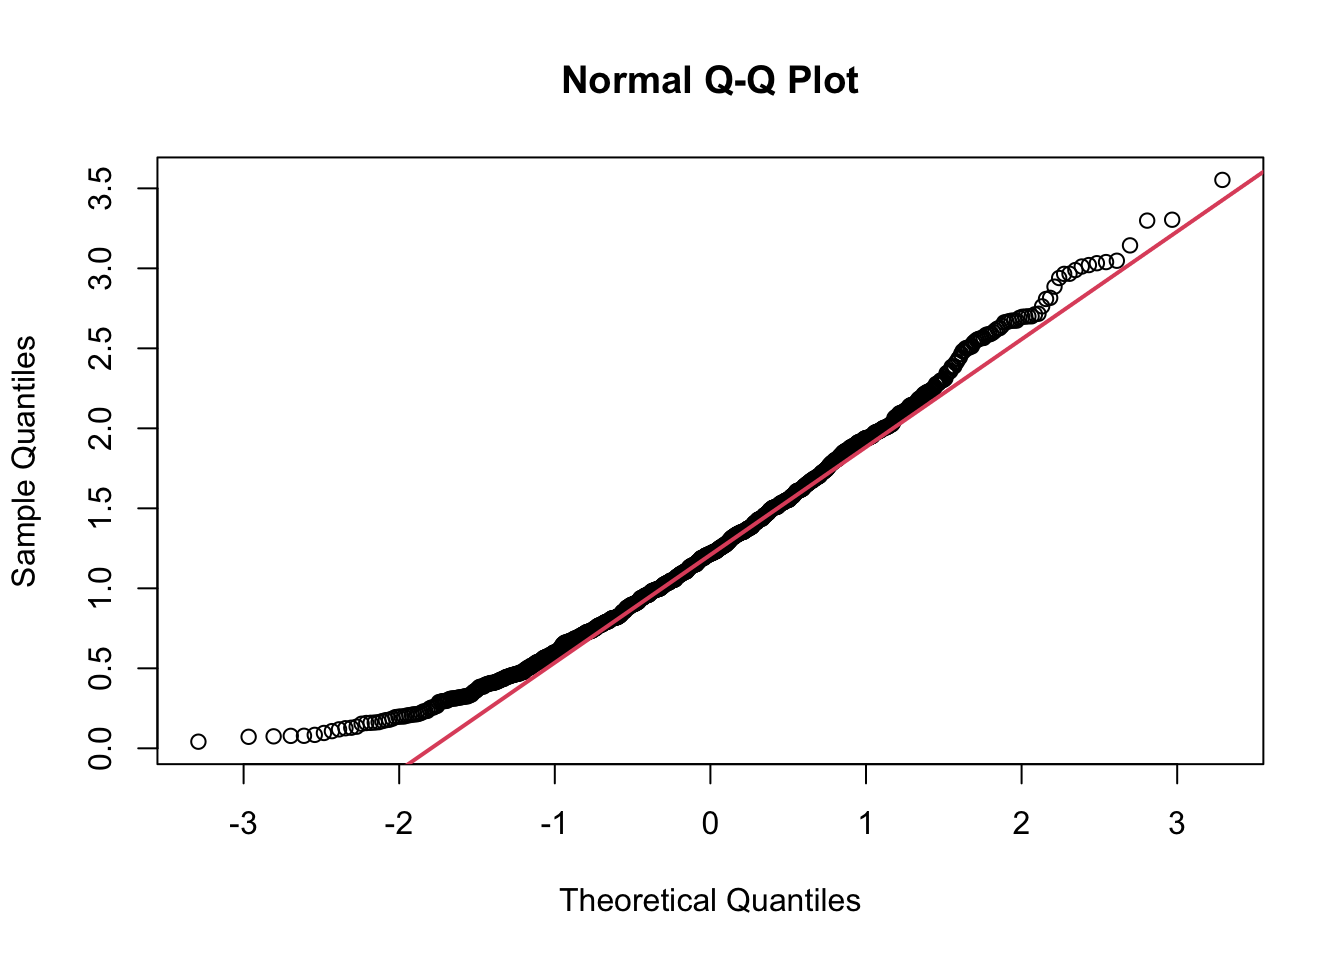
\includegraphics{Question1_Homework1_files/figure-latex/Rayleigh Distribution-1.pdf}

\begin{Shaded}
\begin{Highlighting}[]
\CommentTok{#Histogram of simulated data}
\KeywordTok{hist}\NormalTok{(}\KeywordTok{r}\NormalTok{(}\DecValTok{1000}\NormalTok{,}\DecValTok{1}\NormalTok{), }\DataTypeTok{prob =} \OtherTok{TRUE}\NormalTok{,}\DataTypeTok{xlab =} \StringTok{"Values (Uniform Distribution)"}\NormalTok{,}\DataTypeTok{ylab =} \StringTok{"Frequencies"}\NormalTok{,}\DataTypeTok{main =} \StringTok{"Histogram of Simulated Rayleigh Distribution"}\NormalTok{)}
\end{Highlighting}
\end{Shaded}

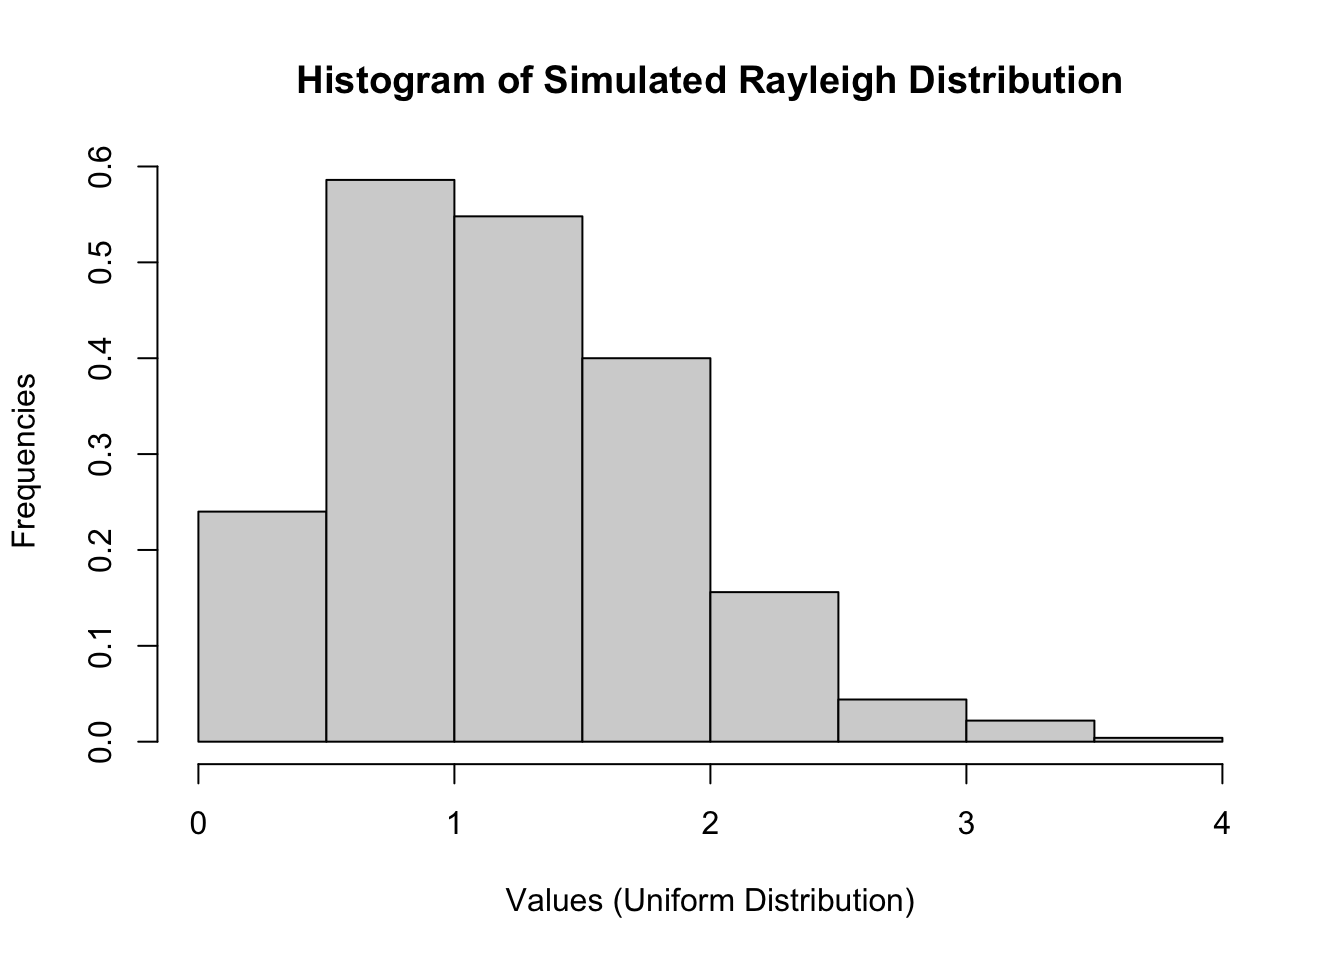
\includegraphics{Question1_Homework1_files/figure-latex/Rayleigh Distribution-2.pdf}

\newpage

\hypertarget{question-3}{%
\section{Question 3}\label{question-3}}

When using Bayesian Inference, we sometimes simulate the prior,
\(\theta\), and maximize it to ensure we are maximizing the mean of the
distribution. This can be done by accepting \(\theta\) as
\(u \le \frac{f(x|\theta)}{f(x|\hat{\theta})}\) where \(u ~ U(0,1)\) and
\(\hat{\theta}\) is the MLE from maximizing \(f(x|\theta)\). Because we
are given the following:

\[u \le \frac{f(x|\theta)}{f(x|\hat{\theta})}\] Based on this equation,
we can simplify the equation through the following proof:
\[u \le \frac{f(x|\theta)}{\int_{}^{\theta}\theta e^{-\theta x}\pi(\theta) d\theta}\]
\$\[$
\]\[
\]\$\$

With this in mind, we can set our equations as follows:

\[f(\theta) = \theta e^{-\theta x}\]
\[g(\theta) = \theta e^{-\theta x}\]
\[M = \frac{\beta^\alpha x^{\alpha - 1} e^{-\beta x}}{\gamma(\alpha)}\]

\begin{Shaded}
\begin{Highlighting}[]
\CommentTok{#Functions}
\NormalTok{theta <-}\StringTok{ }\ControlFlowTok{function}\NormalTok{(x)\{((beta}\OperatorTok{^}\NormalTok{alpha)}\OperatorTok{*}\NormalTok{x}\OperatorTok{^}\NormalTok{(alpha}\DecValTok{-1}\NormalTok{)}\OperatorTok{*}\KeywordTok{exp}\NormalTok{(}\OperatorTok{-}\NormalTok{beta}\OperatorTok{*}\NormalTok{x))}\OperatorTok{/}\KeywordTok{gamma}\NormalTok{(alpha)\}}
\NormalTok{f <-}\StringTok{ }\ControlFlowTok{function}\NormalTok{(theta)\{theta}\OperatorTok{*}\KeywordTok{exp}\NormalTok{(}\OperatorTok{-}\NormalTok{theta}\OperatorTok{*}\NormalTok{x)\}}
\NormalTok{g <-}\StringTok{ }\ControlFlowTok{function}\NormalTok{(theta)}
\NormalTok{m <-}\StringTok{ }\ControlFlowTok{function}\NormalTok{(x)\{(b}\OperatorTok{^}\NormalTok{(a)}\OperatorTok{*}\NormalTok{x}\OperatorTok{^}\NormalTok{(a}\DecValTok{-1}\NormalTok{)}\OperatorTok{*}\KeywordTok{exp}\NormalTok{(}\OperatorTok{-}\NormalTok{b}\OperatorTok{*}\NormalTok{x))}\OperatorTok{/}\NormalTok{(}\KeywordTok{gamma}\NormalTok{(a))\} }\CommentTok{#M is a constant that maximizes the acceptance rejection, so we can take f/g and set it equal to zero to find the maximum value?}
\NormalTok{acceptReject <-}\StringTok{ }\ControlFlowTok{function}\NormalTok{(f,g,alpha,beta,M,n)\{}
\NormalTok{  accept <-}\StringTok{ }\DecValTok{0}
\NormalTok{  X <-}\StringTok{ }\KeywordTok{rep}\NormalTok{(}\DecValTok{0}\NormalTok{,n)}
\NormalTok{  U1 <-}\StringTok{ }\KeywordTok{runif}\NormalTok{(n,}\DecValTok{0}\NormalTok{,}\DecValTok{1}\NormalTok{)}
  \CommentTok{#step1: generate Y and U's}
\NormalTok{  Y <-}\StringTok{ }\NormalTok{g}\OperatorTok{^-}\DecValTok{1}\NormalTok{(U1)}
  \CommentTok{#step2: generate U2 to be a uniform distribution}
\NormalTok{  U2 <-}\StringTok{ }\KeywordTok{runif}\NormalTok{(n,}\DecValTok{0}\NormalTok{,}\DecValTok{1}\NormalTok{) }\CommentTok{#second set of randomly generated values}
  \CommentTok{#Step 3}
\NormalTok{  X =}\StringTok{ }\NormalTok{Y[U2}\OperatorTok{<=}\KeywordTok{f}\NormalTok{(}\KeywordTok{theta}\NormalTok{(Y))}\OperatorTok{/}\KeywordTok{g}\NormalTok{(}\KeywordTok{theta}\NormalTok{(Y))}\OperatorTok{/}\KeywordTok{M}\NormalTok{(Y)]}
  \KeywordTok{return}\NormalTok{(X)}
\NormalTok{\}}

\KeywordTok{set.seed}\NormalTok{(}\DecValTok{500}\NormalTok{)}
\NormalTok{n <-}\StringTok{ }\DecValTok{100}\CommentTok{#number of samples}
\NormalTok{alpha <-}\StringTok{ }\DecValTok{4} \CommentTok{#alpha}
\NormalTok{beta <-}\StringTok{ }\DecValTok{2} \CommentTok{#beta}
\CommentTok{# X <- acceptReject(f,g,alpha,beta,M,n)}
\CommentTok{# hist(X,freq = FALSE, main = paste("Acceptance Rate:",length(X)/n))}
\CommentTok{# xx = seq(min(X),max(X),0.01)}
\CommentTok{# lines(xx,f(xx,xx),col = 'red')#true normal pdf}
\CommentTok{# lines(xx,g(xx)*m(xx),col = 'green')#adjusted pdf}
\end{Highlighting}
\end{Shaded}

\newpage

\hypertarget{question-4}{%
\section{Question 4}\label{question-4}}

\end{document}
